%\documentclass[aps, prl, letterpaper, twocolumn, superscriptaddress, notitlepage, 10pt]{revtex4-1}
\documentclass[aps, prl, letterpaper, twocolumn, superscriptaddress, notitlepage, 10pt]{revtex4}
\usepackage{times}

% use these settings for a more reader-friendly version
%\documentclass[aps, pra, a4paper, 11pt, onecolumn, nofootinbib, superscriptaddress, tightenlines, notitlepage, longbibliography]{revtex4-1}

%------------------------------------------------------------------------------------------------------------%
% Packages
%------------------------------------------------------------------------------------------------------------%

\usepackage{color}
\usepackage{amsmath,amsfonts,amssymb}
\usepackage{graphicx}
\usepackage[caption=false]{subfig}
\usepackage{enumerate}

%\usepackage{tikz}
%\usetikzlibrary{arrows,decorations.pathmorphing,backgrounds,positioning,fit}

\usepackage{epstopdf} % to include .eps graphics files with pdfLaTeX
%\usepackage{bm}  % Define \bm{} to use bold math fonts

\usepackage[pdfpagelabels,pdftex,bookmarks,breaklinks]{hyperref}
\definecolor{darkblue}{RGB}{0,0,127} % choose colors
\definecolor{darkgreen}{RGB}{0,150,0}
\hypersetup{colorlinks, linkcolor=darkblue, citecolor=darkgreen, filecolor=red, urlcolor=blue}
\hypersetup{pdfauthor={Simon Burton, Courtney G. Brell, Steven T. Flammia}}
\hypersetup{pdftitle={Classical Simulation of Quantum Error Correction in a Fibonacci Anyon Code}}

\usepackage[normalem]{ulem}

%------------------------------------------------------------------------------------------------------------%
% Macros
%------------------------------------------------------------------------------------------------------------%

\newcommand{\Eref}[1]{Eq.~(\ref{#1})}
\newcommand{\Fref}[1]{Fig.~\ref{#1}}

\newcommand{\e}{\mathrm{e}}
\newcommand{\vac}{\mathbb{I}}

\newcommand{\ket}[1]{|{#1}\rangle}
\newcommand{\expect}[1]{\langle{#1}\rangle}
\newcommand{\bra}[1]{\langle{#1}|}
\newcommand{\ketbra}[2]{\ket{#1}\!\bra{#2}}
\newcommand{\braket}[2]{\langle{#1}|{#2}\rangle}
\newcommand{\proj}[1]{\ketbra{#1}{#1}}

%------------------------------------------------------------------------------------------------------------%
% Comment fonts
%------------------------------------------------------------------------------------------------------------%

\newcommand{\cggb}[1]{\textcolor{blue}{#1}}
\newcommand{\dude}[1]{\textcolor{red}{#1}}
\newcommand{\stf}[1]{\textcolor{green}{#1}}

%------------------------------------------------------------------------------------------------------------%
\begin{document}

\title{Classical Simulation of Quantum Error Correction in a Fibonacci Anyon Code}

\author{Simon Burton}
\affiliation{Centre for Engineered Quantum Systems, School of Physics, 
The University of Sydney, Sydney, Australia}
\author{Courtney G.\ Brell}
\affiliation{Institut f\"{u}r Theoretische Physik, Leibniz Universit\"{a}t Hannover, 
Appelstra\ss{}e 2, 30167 Hannover, Germany}
\author{Steven T.\ Flammia}
\affiliation{Centre for Engineered Quantum Systems, School of Physics, 
The University of Sydney, Sydney, Australia}

\date{\today}

\begin{abstract}
Classically simulating the dynamics of anyonic excitations in two-dimensional quantum systems is likely intractable in general because such dynamics are sufficient to implement 
universal quantum computation. However, processes of interest for the study of quantum 
error correction in anyon systems are typically drawn from a restricted class that displays 
significant structure over a wide range of system parameters.
We exploit this structure to classically simulate, and thereby demonstrate the success of, an 
error-correction protocol for a quantum memory based on the universal Fibonacci anyon 
model.  We numerically simulate a phenomenological model of the system and noise 
processes on lattice sizes of up to 
$128\times128$ sites, and find a lower bound on the error-correction threshold of 
approximately $12.5\%$, which is comparable to those previously known for abelian and 
(non-universal) nonabelian anyon models.
\end{abstract}

\maketitle

%------------------------------------------------------------------------------------------------------------%

Topologically ordered quantum systems in two dimensions show tremendous promise for 
long-term storage and processing of quantum information~\cite{Kitaev2003, Dennis2002, Nayak2008}. 
The topological features of such systems are insensitive to local 
perturbations~\cite{Bravyi2010, Bravyi2011a, Michalakis2013}, and have quasiparticle excitations 
exhibiting anyonic statistics~\cite{Wilczek1990}. These systems can in general be used as 
quantum memories~\cite{Kitaev2003, Dennis2002} or to perform universal topological 
quantum computation~\cite{Freedman2002, Nayak2008}.

Quantum error correction is vital to harnessing the computational power of topologically 
ordered systems. When coupled to a heat bath at any finite temperature, thermal fluctuations 
will create spurious anyons that diffuse and quickly corrupt the stored quantum 
information~\cite{Pastawski2010}. Thus, the passive protection provided by the mass gap 
at low temperature must be augmented by an \emph{active} decoding procedure. 

In order to efficiently classically simulate an error-correction protocol for 
a topologically ordered quantum memory, it is necessary to simulate 
the physical noise processes, the decoding algorithm, and the physical recovery operations. 
Decoding algorithms are typically designed to run efficiently on a 
classical computer, but there is generally no guarantee that the 
noise and recovery processes should be classically simulable.
Because of this, almost all of the sizable research effort 
on active quantum error correction for topological systems has focused 
on the case of abelian anyons~\cite{Dennis2002, Duclos-Cianci2010, Duclos-Cianci2010a, Wang2010, Wang2010a, Duclos-Cianci2013, Bravyi2011, Bombin2012, Wootton2012, Anwar2014, Watson2014, Hutter2014a, Bravyi2014, Wootton2015, Fowler2015, Andrist2015}.
Systems of abelian anyons are well suited to studying quantum 
error correction because (at the RG fixed point) noise and 
recovery processes can be efficiently simulated numerically, allowing lattice simulations 
of decoding with over 1 million sites~\cite{Duclos-Cianci2010}. 
Standard algorithms are specifically tailored to exploit the abelian nature 
of these particles, particularly that abelian anyons cannot be used for quantum computation. 

Recent investigations have begun to explore quantum error correction for nonabelian anyon 
models~\cite{Brell2013, Wootton2013, Hutter2014, Wootton2015b}. Nonabelian anyon models are especially interesting 
because braiding and fusion of these anyons in general allows for the implementation of universal quantum 
computation. However, the initial studies of error-correction in nonabelian anyon systems have focused on specific models, such as the Ising 
anyons~\cite{Brell2013} and the so-called $\Phi$-$\Lambda$ 
model~\cite{Wootton2013, Hutter2014} that, while nonabelian, are not universal. The general dynamics of these particular anyon models is known to be efficiently classically simulable, a fact
that was exploited to enable efficient simulation of error correction 
in these systems. When considering more general anyon models, their 
ability to perform universal quantum computation would seem a significant 
barrier to their simulation on a classical computer. While simulation 
of general dynamics does indeed seem intractable, we argue that 
the kinds of processes that are typical of thermal noise 
are sufficiently structured  to allow for their classical simulation 
in the regimes where we expect successful error correction to 
be possible. This insight allows us to simulate the noise 
and recovery processes for a quantum code based on a universal anyon model.

Concretely, we consider the simulation of quantum error correction in a two-dimensional lattice 
system with Fibonacci anyons, a class of nonabelian anyons that are universal for quantum 
computation~\cite{Freedman2002, Nayak2008}. Fibonacci anyons are experimentally motivated as the 
expected excitations of the $\nu=\frac{12}{5}$ fractional quantum Hall 
states~\cite{Slingerland2001}, and can be realized in several spin 
models~\cite{Levin2005, Bonesteel2012, Kapit2013, Palumbo2014} and composite 
heterostructures~\cite{Mong2014}.

We use a flexible phenomenological model of dynamics and thermal 
noise to describe a system with Fibonacci anyon excitations. Within 
this model, we apply existing general topological error-correction protocols, and 
simulate the successful preservation of quantum information encoded in topological 
degrees of freedom. Topological quantum computation protocols using nonabelian anyons 
typically implicitly assume the existence of an error-correction protocol to 
correct for diffusion or unwanted creation of anyons. Our results 
are the first explicit demonstration that such a scheme will 
be successful when applied to a universal topological quantum computer.

%------------------------------------------------------------------------------------------------------------%
%\paragraph{Modeling Fibonacci anyons.}
%\paragraph{Topological quantum field theory.}
\paragraph{Topological model.}

%The topological features of a physical anyon model are abstractly described by a unitary 
%modular tensor category~\cite{Wang2010b}. This object contains the data describing the 
%types of anyonic particles, as well as the results of topological operations such as braiding and 
%fusion of these anyons. The Fibonacci anyon model consists of only one non-trivial particle 
%type, conventionally labelled $\tau$. Denoting the vacuum by $\vac$, we can describe 
%the possible fusion outcomes of Fibonacci anyons as $\tau\times\tau=\vac+\tau$, 
%i.e.~two $\tau$ particles can either fuse to vacuum or to a $\tau$ particle.
%
%Associated with each set of fusion outcomes for a fixed number of $\tau$ particles is a basis 
%vector for a Hilbert space, the \emph{fusion} space. For $n$ particles of type $\tau$, the 
%dimension of this space grows asymptotically as $\varphi^n$ for $\varphi=\frac{1+\sqrt{5}}{2}$ 
%the golden ratio. Additionally, there is a global degeneracy associated with the topology of the 
%manifold on which the anyons reside. We will consider systems with the topology of a torus, 
%which for the Fibonacci anyons gives rise to a 2-fold degeneracy. For convenience 
%(in particular to minimize finite-size effects in our numerical computations~\cite{Brell2013}), 
%this global space is the one in which we will encode, and demonstrate protection of, quantum 
%information.
%
%The fusion outcome of any particular experiment depends on the history of the particles, in 
%particular how they have braided around one another. Braiding operations are treated as 
%unitary actions on the fusion space. Pair-creation events should be considered isometries 
%that enlarge the fusion space, while fusion events correspond to projective measurements 
%of combined charge of some number of particles. For detailed description of these 
%processes in Fibonacci anyons, see e.g.~Ref.~\cite{Nayak2008} and references therein. 
%Braiding of Fibonacci anyons and measurements of fusion outcomes is known to be 
%sufficient to implement universal quantum computation~\cite{Freedman2002, Nayak2008}.


% From Picture TQFTs paper:
%Within physics, TQFTs are referred to as “anyonic systems” [Wil][DFNSS]. These are
%2-dimensional quantum mechanical systems with point like excitations (variously
%called “quas-particle” or just “particle”, anyon, or perhaps “nonabelion”) which
%under exchange exhibit exotic statistics: a nontrival representation of the braid
%groups acting on a finite dimensional Hilbert space V consisting of “internal de-
%grees of freedom”. Since these “internal degrees of freedom” sound mysterious,
%we note that this information is accessed by fusion: fuse pairs of anyons along
%a well defined trajectory and observe the outcome.
%Statistics of anyons is described by unitary representations of the braid groups

We consider a 
2-dimensional system with
point-like excitations or quasiparticles known as anyons.
These anyons show exotic statistics under exchange.
The worldlines of these exchanges form \emph{braids}
in (2+1)-dimensions
which act unitarily on (the Hilbert space of) degrees of freedom known as the \emph{fusion space.}
To access this space we define
the topological observables of the system: these
are total charge measurements within regions bounded by closed loops (Wilson loops).
%The algebraic properties of these processes
These dynamics and observables obey algebraic rules
given by a unitary modular tensor category~\cite{Wang2010b}. % (UMTC). 

%As was noted in~\cite{Pfeifer2014}, when dealing with two-dimensional 
%anyon dynamics, it is not sufficient to consider only
%the algebraic (fusion/braiding) properties of the anyons,
%one must also account for the algebra of observables. \cggb{This sentence seems odd here. Consider moving?}

From the perspective of
\emph{topological quantum field theory}
anyons are modelled
as punctures in a surface~\cite{Pfeifer2014}, and it is not
the anyons themselves that braid, but the manifold in which the anyons reside 
becomes deformed (twisted) by these braid moves.
This is the perspective we adopt.
In particular, this shows the action of braiding
on arbitrary observables (Wilson loops) as
these deform with the manifold.

The state of a collection of anyons
can be described by the observables of the system.
The difference between abelian and non-abelian
anyon theories is that the outcomes of measurements in an abelian theory
are determined uniquely particle content only.
That is, the fusion space is one-dimensional for abelian anyons, and generally larger for non-abelian anyons.
%An example is Fibonacci: $\tau\times\tau=\tau+\vac$
%\emph{picture here?}
%specify a state requires nesting multiple wilson lines.
In particular, we consider a system supporting (non-abelian) Fibonacci
anyon excitations, denoted by $\tau.$
Two such anyons can have total charge
that is a superposition of $\tau$ and $\vac$ (vacuum),
so the fusion space in this case is 2-dimensional.
We can represent basis states for this space using diagrams of definite total charge for the Wilson loops, and arbitrary states as linear combinations of these diagrams:
\begin{align*}
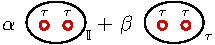
\includegraphics[]{pic-fibonacci.pdf}
\end{align*}

For $n$ anyons of type $\tau$, the 
dimension of this space grows asymptotically as $\varphi^n$ for $\varphi=\frac{1+\sqrt{5}}{2}$ 
the golden ratio. Additionally, there is a global degeneracy associated with the topology of the 
manifold on which the anyons reside. We will consider systems with the topology of a torus, 
which for the Fibonacci anyons gives rise to a 2-fold degeneracy.
%For convenience 
%(in particular to minimize finite-size effects in our numerical computations~\cite{Brell2013}), 
This global space is the one in which we will encode, and demonstrate protection of, quantum 
information. 

Observables associated to non-intersecting loops commute, and so
a basis for the space can be built from a maximal
set of disjoint, nested loops.
For three anyons, two
possible ways of nesting loops are related %these measurements
via $F$-moves:
\begin{align}
\label{e:fmove}
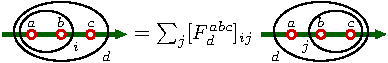
\includegraphics[]{pic-fmove.pdf}
\end{align}
Here we have shown particles with charges $a$, $b$, and $c$
as well as total charge $d$.
The lefthand side shows a state where the anyons with charge $a$ and $b$ are
observed to have total charge $i$.
The righthand side involves a superposition 
over total charge $j$ of the anyons with charge $b$ and $c$.
The green line serves to linearly
order the anyons, and track
deformations in the underlying space 
(the history of braiding processes).
It also denotes the direction along
which $F$-moves occur.

%Here we show how braids effect observables:
%Here we show the $R$-move, corresponding to a (clockwise) braiding processes:
A clockwise braiding process is represented by an $R$-move:
\begin{align}
\label{e:rmove}
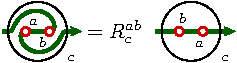
\includegraphics[]{pic-rmove.pdf}
\end{align}
%where $a$, $b$, and $c$ represent particle types, and $F$-moves,
%representing the associativity rule for fusion processes, 
This is meant to show a \emph{half-twist} of the space
inside the observable with value $c$
holding two anyons (punctures) with charges $a$ and $b$.
We are free to draw loops around charges,
and in general braiding will twist these loops in different
ways:
\begin{align*}
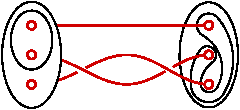
\includegraphics[]{pic-braid-loop.pdf}
\end{align*}
%
%
These diagrams can be composed, and the fusion operation replaces the 
interior of a disc by a single charge.
These pictures, abstracted from the quantum context,
are called \emph{curve diagrams} and are used in
the study of braid groups \cite{Dehornoy2002}.
%In general, such a curve diagram is 
%a continuous embedding of a line that passes through 
%each puncture once. 
%Remarkably, any two such linear orderings are related by
%braiding (half-twists).
%\dude{optional paragraph..}

For the Fibonacci anyons, the non-trivial $R$ and $F$ moves are 
\begin{equation*}
	R_{\vac}^{\tau\tau} = \e^{\frac{-4\pi i}{5}} 
	\ \ , \ \
	R_\tau^{\tau\tau}= \e^{\frac{3\pi i}{5}} 
	\ \ , \ \
	F_{\tau}^{\tau\tau\tau} = \begin{pmatrix}\varphi^{-1}&\varphi^{-\frac{1}{2}}\\\varphi^{-\frac{1}{2}}&-\varphi^{-1}\end{pmatrix} \,,
\end{equation*}
where the matrix is given in a basis labelled $(\vac,\tau)$.
%unitary actions on the fusion space. Pair-creation events should be considered isometries 
%that enlarge the fusion space, while fusion events correspond to projective measurements 
%of combined charge of some number of particles.
For detailed description of these 
processes in Fibonacci anyons, see e.g.~Ref.~\cite{Nayak2008} and references therein. 
Braiding of Fibonacci anyons and measurements of fusion outcomes is known to be 
sufficient to implement universal quantum computation~\cite{Freedman2002, Nayak2008}.

This treatment of anyon dynamics we consider to be a phenomenological model;
it neglects any microscopic details of the system.
This is consistent with the principles of topologically 
ordered systems and anyonic physics, where the key universal features describing the 
anyon model correspond to large length-scale physics, while the microscopic physics plays 
a less important (and non-universal) role.

%We use a phenomenological model of Fibonacci anyon dynamics which neglects any 
%microscopic details of the system. 
%This is consistent with the principles of topologically 
%ordered systems and anyonic physics, where the key universal features describing the 
%anyon model correspond to large length-scale physics, while the microscopic physics plays 
%a less important (and non-universal) role.
%Our simulation is in effect that of a $(2+1)$-dimensional topological 
%quantum field theory, which allows for topological processes such as 
%pair-creation, braiding, and fusion of anyonic charges. 

%------------------------------------------------------------------------------------------------------------%
\paragraph{Noise and error-correction.}

%We model the system on a periodic $L\times L$ square lattice $\Lambda$ of \emph{tiles} on which anyons can reside. 
%This treatment applies equally well to lattice models, where anyons 
%can only be located at a discrete set of points, 
%or continuum models, where a discretization of the manifold must 
%be chosen in order to perform charge measurements. 
%In the former case, each tile of $\Lambda$ represents a 
%lattice site, while in the latter case each tile represents 
%a measurement region. For more details of an analogous model, see~\cite{Brell2013}.

We consider encoding a qubit of quantum information in the global degeneracy associated 
with the topology of the manifold of our system.
We endow this manifold with a finite set of $L\times L$ observables arranged in
a square lattice tiling $\Lambda$.
These \emph{tiles} will be the oservables accesible to the error-correction procedure (\emph{decoder}).
We can use these observables to construct an idealized Hamiltonian for this system of the form
\begin{align}
	H=-\sum_{T\in \Lambda}\proj{\vac}_T\;,\label{e:hamiltonian}
\end{align}
with $\proj{\vac}_T$ the projector to charge $\vac$ at tile $T$, i.e.~the ground 
space of the model has vacuum total charge in each tile.
Given the toroidal boundary 
conditions, this space contains the two-fold degenerate codespace.
%We identify this ground space as the codespace of our model. 
Typical realistic noise processes in this kind of system are 
pair-creation, hopping, exchange etc.~of anyons on neighboring sites of $\Lambda$.
It was seen in~\cite{Brell2013} that a simplified noise model consisting of pair-creation events only 
is sufficient to capture the qualitative features of an error-correction simulation, and so for convenience we 
will restrict to pair-creation noise processes in the numerical results presented in this study. 
Such pair-creation events act on neighboring pairs of sites,
and so may be associated with an edge of the lattice, chosen 
uniformly at random at each time step of the simulation. The simulation time, and thus the 
error-correction threshold, will be measured in terms of average number of noise processes 
per edge, as opposed to an iid noise probability per edge. The latter measure is not 
appropriate for error processes in nonabelian anyon models, but the two coincide in the limit 
of low error rates in those cases where they are comparable (see Ref.~\cite{Brell2013}).

In order to perform a logical error on our code, a noise process must have support on a 
a homologically nontrivial region of the lattice.
These correspond to processes in which anyonic charge is transported around a non-trivial loop before 
annihilating to vacuum.

Our error-correction algorithm is
based on a hierarchical clustering algorithm~\cite{Hastie2009, Wootton2015b},
and follows a similar strategy to the hard-decision renormalization group decoder~\cite{Bravyi2011}. 
The decoder proceeds by measuring the occupations of 
anyons at each site of the lattice, producing a \emph{syndrome} 
of occupied sites. Following this, it forms clusters of nearby anyons and 
measures the total charge within each cluster.
Clusters with trivial charge are discarded, and
the rest are joined (agglomeratively~\cite{Hastie2009})
at linearly increasing length scales. This iterative process concludes when 
there is at most a single cluster remaining (see \Fref{f:decode}).
Note that unlike the case of abelian anyons, the decoder
cannot determine the charge of each cluster given only the syndrome information (as in \cite{Bravyi2011}),
and so will query (measure) the system to find this.
Our simulation proceeds in this way as a dialogue between decoder
and system, terminating when either the decoder itself terminates or 
when it performs a homologically nontrivial operation, thereby altering the 
codespace (and failing to perform successful information recovery).
Note that, as was found in Ref.~\cite{Brell2013}, we expect that 
our qualitative results may be reproduced by most alternative families 
of decoders, although it may not be clear in all cases how to extend these decoders to the non-abelian setting.
The advantage of using a clustering decoder is 
its simplicity and flexibility, and the fact that its clustering 
scheme is compatible with the structure in the noise 
processes that allows us to classically simulate them.

\begin{figure}[t!]
\begin{center}
	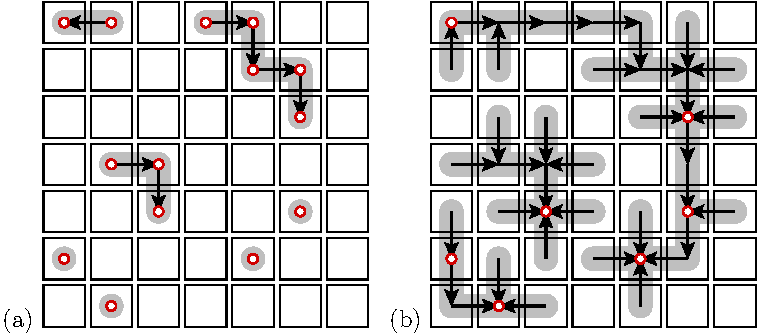
\includegraphics[width=1.0\columnwidth]{pic-decode.pdf}
\caption{The decoder works by maintaining a set of disjoint clusters as rooted trees.
(a) At the initial clustering stage, these trees are formed 
from neighboring sites that contain charges. Within each cluster, the 
charges are transported to the root of the tree (chosen 
arbitrarily), and their combined charge measured. The direction of transport 
(towards the root) is denoted by arrows.
(b) At each successive round, all trees are grown in 
every direction, and overlapping trees are joined. Again, any charges 
within a cluster are transported to the root of the 
tree and measured. All clusters with vacuum total charge are deleted.
\label{f:decode}
}
\end{center}
\vspace{-10pt}
\end{figure}

%------------------------------------------------------------------------------------------------------------%	
\paragraph{Classical simulability.}

Although simulating pair creation, braiding, and fusion of $n$ Fibonacci anyons is equivalent 
in computational power to universal quantum computing (and thus unlikely to be classically 
tractable), noise processes and error-correction procedures have structure that we can 
exploit to efficiently simulate typical processes of interest. In particular, those 
processes in which we expect error-correction to succeed are also those that we expect to 
be able to efficiently simulate for the following heuristic reasons 
(we leave a more rigorous analysis of simulability for noise 
and error correction processes as an open problem).

Below the (bond) percolation threshold for (say) a 2D square lattice, we expect random sets of 
bonds to decompose into separate connected components 
of average size $O(\log(n))$ and variance $O(1)$~\cite{Bazant2000}.
Each noise process in our model is associated with a (randomly distributed) edge, and so 
disconnected components correspond to sets of anyons that could not have interacted at any 
point in their history. 
We are free to neglect the degrees of freedom associated with braiding between components 
because each component has trivial total charge.
This allows us to simulate the braiding processes within each component separately. 
In other words: the quantum state in the fusion space of all anyons factorizes into 
a tensor product over components. 
Since each 
component has size only $O(\log(n))$, we can typically simulate these dynamics efficiently 
because the resulting fusion space has dimension $O(\mathrm{poly}(n))$. 
There are 
random processes that violate this reasoning, but processes such as these are suppressed 
exponentially in the lattice size $L$~\cite{Grimmett1989}. 

However, random noise processes are not the only dynamics that we need to consider. We 
must also consider the effect of the error-correction routine itself. This acts iteratively to fuse 
particles on increasing length scales. While this kind of fusion would typically merge components, 
forcing us to compute dynamics of larger and larger sets of anyons,
large components are sparsely distributed 
(and thus unlikely to be merged), and in addition at each length scale the total number of 
anyons present is dramatically reduced by fusion, leading to a smaller number of anyons that 
must be simulated.

At some point, with strong enough noise, the state will
no longer decompose at all and computing dynamics will
become exponentially difficult in the system size.
However, for finite lattice size, we use heuristics
to minimize non-local braid moves, which helps to
maintain the state as a separable product.
This enables simulation of error correction in
the area around decoder threshold for lattice sizes up to $L=128.$
%However, for finite lattice size, this regime is somewhere
%beyond the decoder threshold, which is the 
%point at which the decoder creates nontrivial (extensive) loops.
%\stf{CGB and I are still not confident in the previous sentence or the next one}
%We can view the system state as a tensor network, on which
%the decoder is performing an (efficiently simulable) contraction.
%This enables simulation of error correction in
%the area around decoder threshold for lattice sizes up to $L=128.$
%\dude{more polish needed...}

%However, recall that logical errors in our system correspond to 
%processes that act over a non-trivial loop of the torus. 
%Below the point at which the decoder begins to create 
%such nontrivial loops, our simulation remains efficient
%while it begins to declare failure whenever non-trivial logical 
%operations occur. This allows us to simulate large lattice sizes 
%in the successful error-correction (sub-percolated) regime, including up to $L=128$.

%------------------------------------------------------------------------------------------------------------%	
\paragraph{Simulation algorithm.}

%Our concrete simulation proceeds by associating a tile with each site of the 
%$L\times L$ periodic square lattice $\Lambda$.

%In order to keep track of the state of the system we maintain a set of disjoint curves, 
%\cggb{do they need to be directed, or is that just for the figure?} 
%representing the history of anyons on the lattice.
%These curves can also be thought of as a top-down view of the fusion tree:
%the anyons comprising the fusion tree are here displayed as points along each curve. 
%In general, the curves wind around our two 
%dimensional manifold in a haphazard way determined by the progress of the simulation.
%This creates a dynamically generated basis for the fusion space 
%that easily allows for tensor factorization of disjoint components. 
%For comparison, previous work used a single fixed basis for 
%the fusion space determined by row-major ordering of sites~\cite{Brell2013}.

In order to keep track of the state of the system we maintain 
a set of disjoint directed curves, 
one for each connected component with trivial total charge.
The application of a pair-creation noise process corresponds to the 
addition of an extra piece of curve to the lattice supporting
two new anyons.
%along with two preferred points on it denoting the anyon locations. 
Following the noise processes, our simulation must %proceed to 
measure the total charge within each tile; the results of 
these measurements will form the error syndrome. 
This requires joining (arbitrarily) any curves that intersect that tile, 
and then performing $R$ and $F$-moves on the resulting
curve so that 
all anyons within the tile have been 
localized within a contiguous region of the curve. 
%\dude{Heisenberg picture?}
%The observable corresponding to the tile is then
%represented in the state \dude{polish}.
%The total charge is then (probabilistically) read off the 
%relevant section of the fusion tree. 
An example of this 
procedure for a simple noise process is shown in \Fref{f:syndrome}.
%and the corresponding braid moves are shown in \Fref{f:syndrome}(e).
The combinatorial derivation of the algorithm and data structures used for 
this procedure will be discussed elsewhere.
%Braiding processes that encircle 
%a non-trivial loop of our (toric) manifold can also be 
%treated in an analogous way, following e.g.~\cite{Pfeifer2012}.
%\cggb{This paragraph and the next still needs another look.}

\begin{figure}[t!]
\begin{center}
	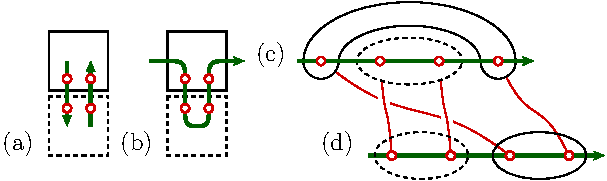
\includegraphics[width=1.0\columnwidth]{pic-syndrome.pdf}
\caption{
(a) Noise processes initially form isolated sets of pair-created anyons, 
each crossing the boundary of a tile. 
(b) To measure the total charge 
contained within each tile, 
we first join the participating curve 
diagrams arbitrarily into a single curve diagram.
(c) The total charge of each tile can then be found 
by braiding anyons around each other until all charges within 
a tile are neighbors on the curve, as in (d).  
The red lines correspond to the worldline braids that perform this step.
}
\label{f:syndrome}
\end{center}
\vspace{-10pt}
\end{figure}

Following the result of these charge measurements, the decoder determines 
a recovery operation that involves fusion of subsets of anyons. 
These fusion results can be calculated in the same way, 
and the output charge placed at an appropriate point in the lattice. 
This procedure is iterated until either the decoder terminates successfully, 
or the simulation itself declares failure.


%------------------------------------------------------------------------------------------------------------%
\paragraph{Numerical results.}

We plot the performance of the decoder as a function of error rate for varying lattice sizes in 
\Fref{f:threshold}. 
The error rate is parameterized by the Poisson process duration $t_{\mathrm{sim}}$, representing the expected number of errors per edge during the simulation. 
We find evidence of a decoding threshold below which decoding succeeds with asymptotic 
certainty as the system size increases at $t_{\mathrm{sim}}\simeq 0.125 \pm 0.003$.

\begin{figure}[t!]
\begin{center}
	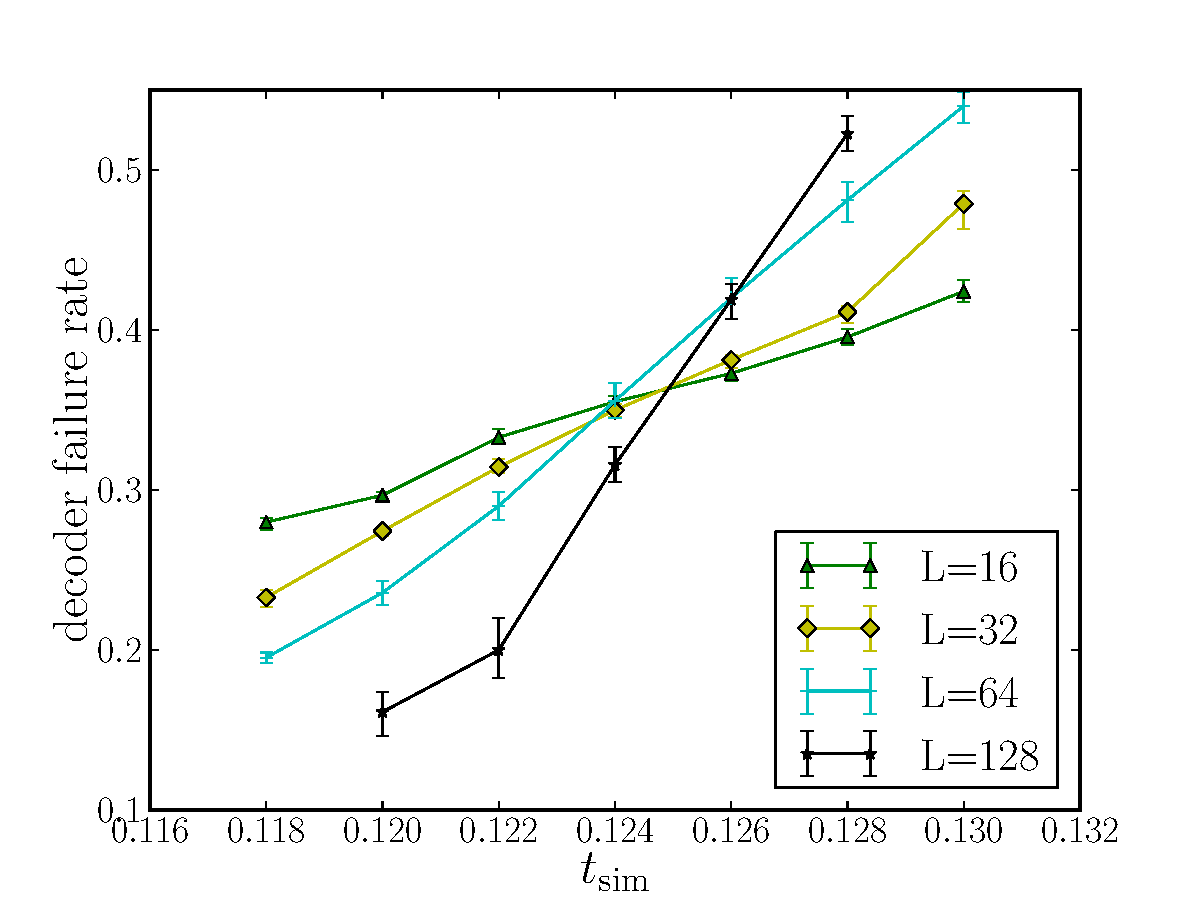
\includegraphics[width=\columnwidth]{anyons-kyle.pdf}
\caption{The decoder failure rate (a lower bound on the logical error probability) is shown as a function of simulation time for linear lattice sizes from $L=16$ to $128$. 
This exhibits threshold behavior at a critical memory lifetime of $t_{\mathrm{sim}}^*\simeq 0.125$. 
This implies the Fibonacci anyon code simulated here is able to perfectly reliably store quantum information for times less than $t_{\mathrm{sim}}^*$ in the $L\to \infty$ limit.}
\label{f:threshold}
\end{center}
\vspace{-10pt}
\end{figure}

We can guarantee that error-correction will succeed whenever
the action of noise plus decoder 
does not percolate the anyons accross the lattice,
but it is possible that percolated events may still result in no error. 
The connection between the percolation threshold and the error-correction threshold 
is not well understood in general~\cite{Hastings2014}, though it is clear 
that our threshold estimate will be a lower bound for 
the true threshold that may be found if all events 
(including those that have percolated) were simulated by an optimal decoder. 
However, calculations of such nontrivial operations suggest that all such 
processes will indeed result in a logical or leakage error.
As such it is likely that neglecting full simulation for 
such events does not significantly affect our observed threshold value.

%------------------------------------------------------------------------------------------------------------%
\paragraph{Discussion.}

We have demonstrated classical simulation of successful error correction in a universal anyon model. 
Though we have chosen several properties of our model and 
simulation in a convenient way for simplicity,
Ref.~\cite{Brell2013} presents good evidence that it is
unlikely that these choices will affect our results qualitatively.
%it seems highly
%unlikely that they will affect the qualitative results, similarly to the results of Ref.~\cite{Brell2013}. 
In particular, although we have modeled our logical qubit as 
encoded in the global topological degrees of freedom of our 
system, we could have encoded it in the fusion space of several preferred anyons. 
This situation would be appropriate to model error-correction routines for topological quantum computation. 
Additionally, we expect our results to be stable to changes in details of the noise model and decoding algorithm.

None of our techniques are restricted to simulation of Fibonacci anyon dynamics, and could 
equally well be used to simulate successful error-correction protocols in an arbitrary anyon code. 
As such, our methods could be used to demonstrate successful 
error-correction in an arbitrary anyonic topological quantum computation.

There are several interesting avenues for further research. 
Although it is not completely obvious how to do so, 
applying these methods to more realistic models such as concrete 
microscopic spin models or models with non-topological features would give 
direct insight into practical error rates needed for topological quantum memories in non-Abelian systems. 
It would be extremely interesting to find \emph{classical} spin models 
whose phase diagram encodes the threshold for error correction in these systems~\cite{Dennis2002}.
%Another potential direction is to incorporate tensor network methods for 
%simulating anyons~\cite{Pfeifer2012, Singh2014} to improve the speed and scale of the simulations. 
Finally, perhaps the most important open question is whether 
\emph{fault-tolerant} decoders can be designed for nonabelian anyon codes. 


%------------------------------------------------------------------------------------------------------------%
\acknowledgments 

We thank A.\ Doherty and R.\ Pfeifer for discussions. 
This work was supported by the ARC via EQuS project number CE11001013, by the US Army Research Office grant numbers W911NF-14-1-0098 and W911NF-14-1-0103, ERC grant QFTCMPS and by the cluster of excellence EXC 201 Quantum Engineering and Space-Time Research. STF also acknowledges support from an ARC Future Fellowship FT130101744.

%------------------------------------------------------------------------------------------------------------%
\bibliography{refs2}

\end{document}
